\chapter{Webová aplikace}
V~této kapitole budou představeny jednotlivé aplikace, jejich funkce a způsob integrace s~vyvinutými nástroji framesss a desssign.

Webová aplikace, vyvinutá v~rámci projektu \textit{Vývoj komplexního softwaru pro optimalizaci návrhu a posouzení střešních a stropních konstrukcí}, zahrnuje dvě hlavní aplikace: STŘECHA a STROP. Tato kapitola popisuje jednotlivé aplikace, jejich funkce a integraci s~vyvinutými knihovnami framesss a desssign.

Aplikace slouží pro předběžné ověření dimenzí konstrukčních prvků s~využitím řešení a výrobků společnosti Wienerberger.

Kromě integrace knihoven představených v~předcozích kapitolách bylo v~rámci této diplomové práce vyvinuté nové uživatelské prostředí. Z~časových důvodů bylo implementováno zatím pouze do aplikace STŘECHA. Aplikaci STROP tento přechod čeká v~nejbližší době.

Webová aplikace zatím nemá stanovenou doménu, proto je přístupná přes přesměrování z~adresy \url{https://people.fsv.cvut.cz/www/holanjak/software/wienerberger}.

\section{Aplikace STŘECHA}
Aplikace STŘECHA je určena pro předběžný návrh konstrukčních prvků krovu se střešními krytinami a skladbami Tondach. V~rámci této diplomové práce došlo k~výraznému zlepšení grafického uživatelského rozhraní a interakce s~uživatelem.

\subsection{Původní verze aplikace}
Původní verze aplikace STŘECHA poskytovala základní nástroje pro posouzení krovů. Uživatel procházel jednotlivými kroky, od zadání geometrie objektu, přes zadání lokality pro výpočet klimatických zatížení, zvolení krytiny, skladby střešního pláště, až po definování průřezů a materiálů jednotlivých prvků. Následně byla takto zadaná konstrukce posouzena na několik předem definovaných kombinací zatížení, které uživatel nemohl upravit.

Původní uživatelské prostředí bylo tvořeno několika velkými statickými formuláři, který byly sice přehledné, ale velmi dlouhé. Uživatelé zároveň neměli žádnou vizuální kontrolu nad tím, co zadávají, což mohlo vést k~chybám při zadávání dat. Výsledky byly prezentovány ve formě textového výstupu, ve velmi stručné formě, což omezovalo možnosti interaktivní zpětné vazby.

\begin{figure}[H]
    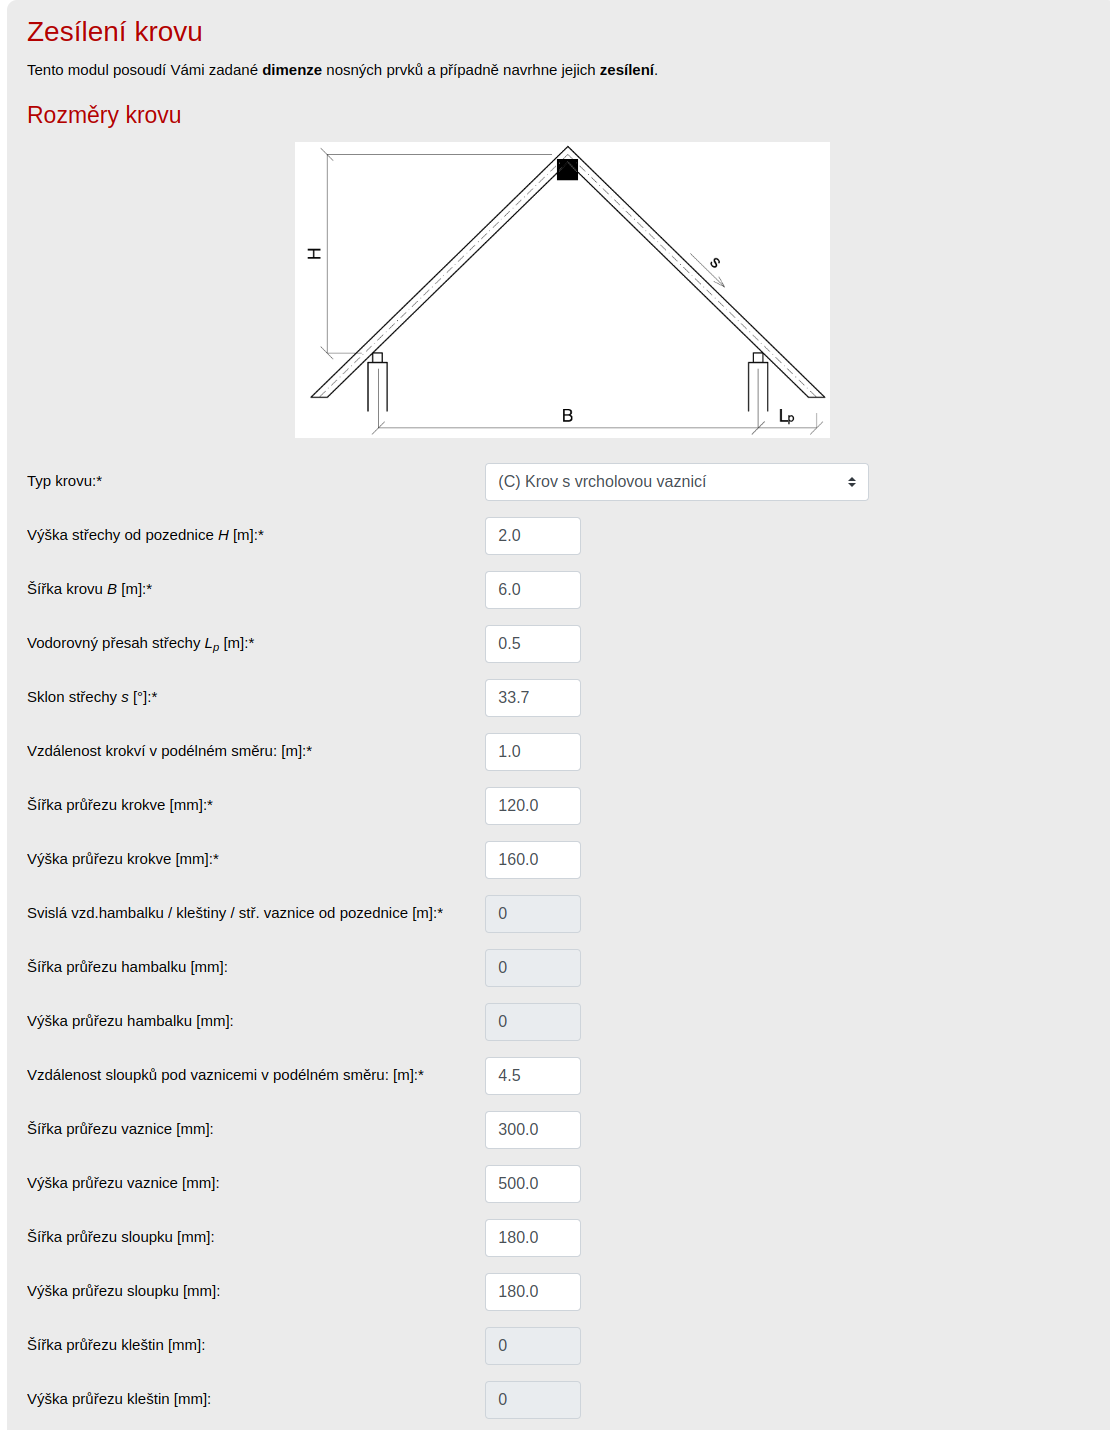
\includegraphics{assets/figures/wbapp/strecha_old-0-0.png}
    \caption{STŘECHA -- Modul pro finální posouzení 1/2}
    \label{fig:roof_old_1}
\end{figure}

\begin{figure}[H]
    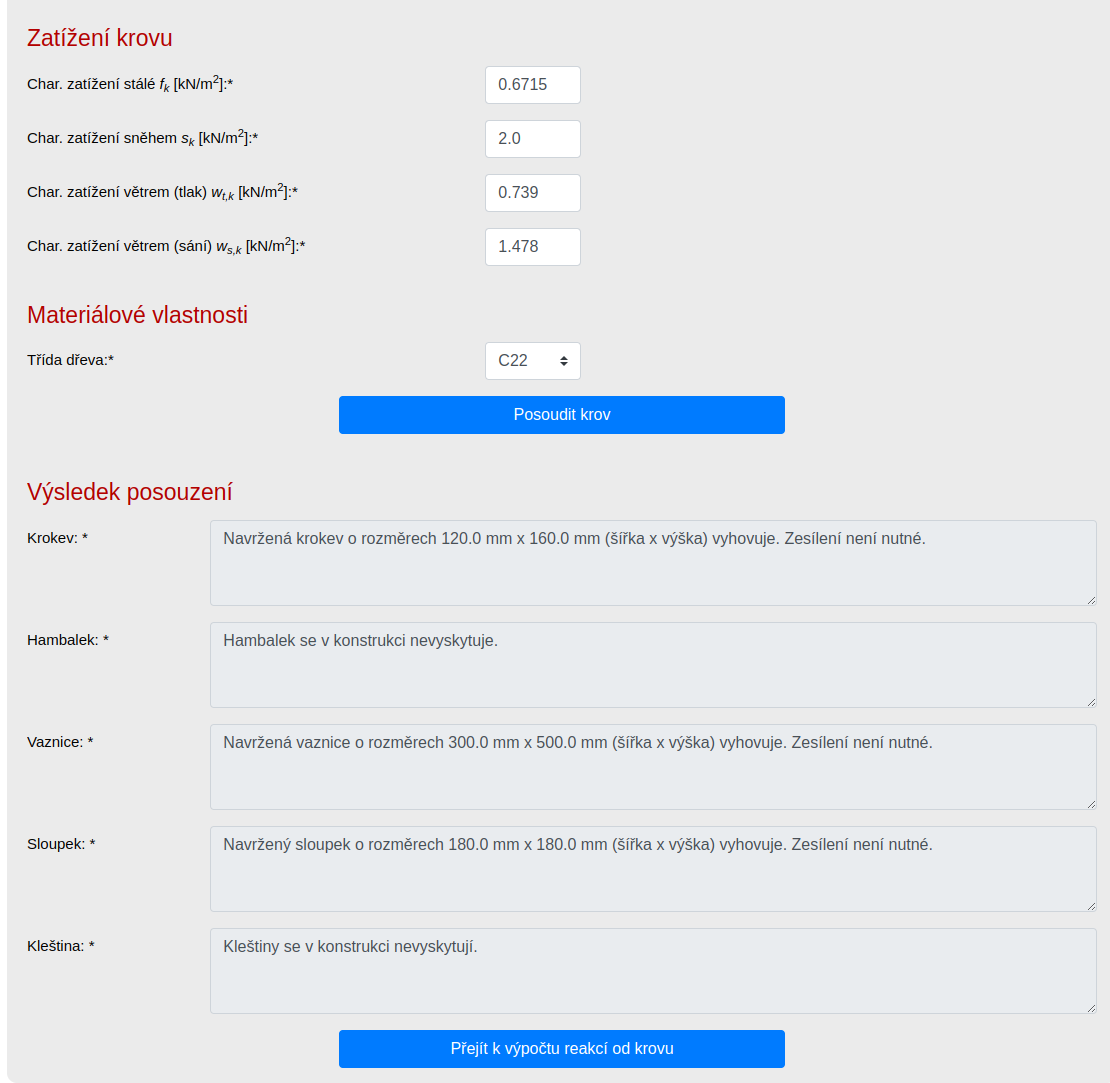
\includegraphics{assets/figures/wbapp/strecha_old-0-1.png}
    \caption{STŘECHA -- Modul pro finální posouzení 2/2}
    \label{fig:roof_old_2}
\end{figure}


\subsection{Nová verze}
Nová verze aplikace STŘECHA přináší výrazné zlepšení v~uživatelském rozhraní a interaktivitě. Používá moderní technologie pro dynamickou vizualizaci a umožňuje uživatelům interaktivně modelovat střešní konstrukce.

\subsubsection*{Funkčnost}
Nová verze aplikace STŘECHA umožňuje uživatelům projít několika kroky k~vygenerování statického schématu se zatíženími a zatěžovacími stavy, podobně jako tomu bylo v~původní verzi. Nově však uživatel může měnit geometrii, přidávat a ubírat zatížení, definovat zatěžovací stavy, kombinovat je do kombinací a zobrazovat si výsledky pro jednotlivé stavy zvlášť.

Pro všechny tyto funkce aplikace využívá knihovny framesss a desssign, které byly představeny v~předchozích kapitolách.

\subsubsection*{Uživatelské prostředí}
Nové uživatelské prostředí aplikace STŘECHA nabízí intuitivní a interaktivní rozhraní, které uživatelům umožňuje snadno zadávat data a mít nad nimi vizuální kontrolu.

V~hlavní části obrazovky se nachází vizualizace modelu střechy, kde jsou zobrazeny uzly, prvky a aplikovaná zatížení. Uživatel může interaktivně přidávat uzly, prvky a zatížení pomocí ovládacích prvků v~dolní části obrazovky. Tento přístup zajišťuje, že uživatelé mají přehled o~všech zadaných datech a mohou je snadno upravovat a kontrolovat.

Uživatel může v~prostředí aplikace:
\begin{itemize}
    \item generovat střešní konstrukci z~předdefinovaných typů střešních konstrukcí,
    \item přidávat, editovat a mazat entity,
    \item vypočítat vnitřní síly,
    \item posoudit konstrukci.
\end{itemize}

\begin{figure}[H]
    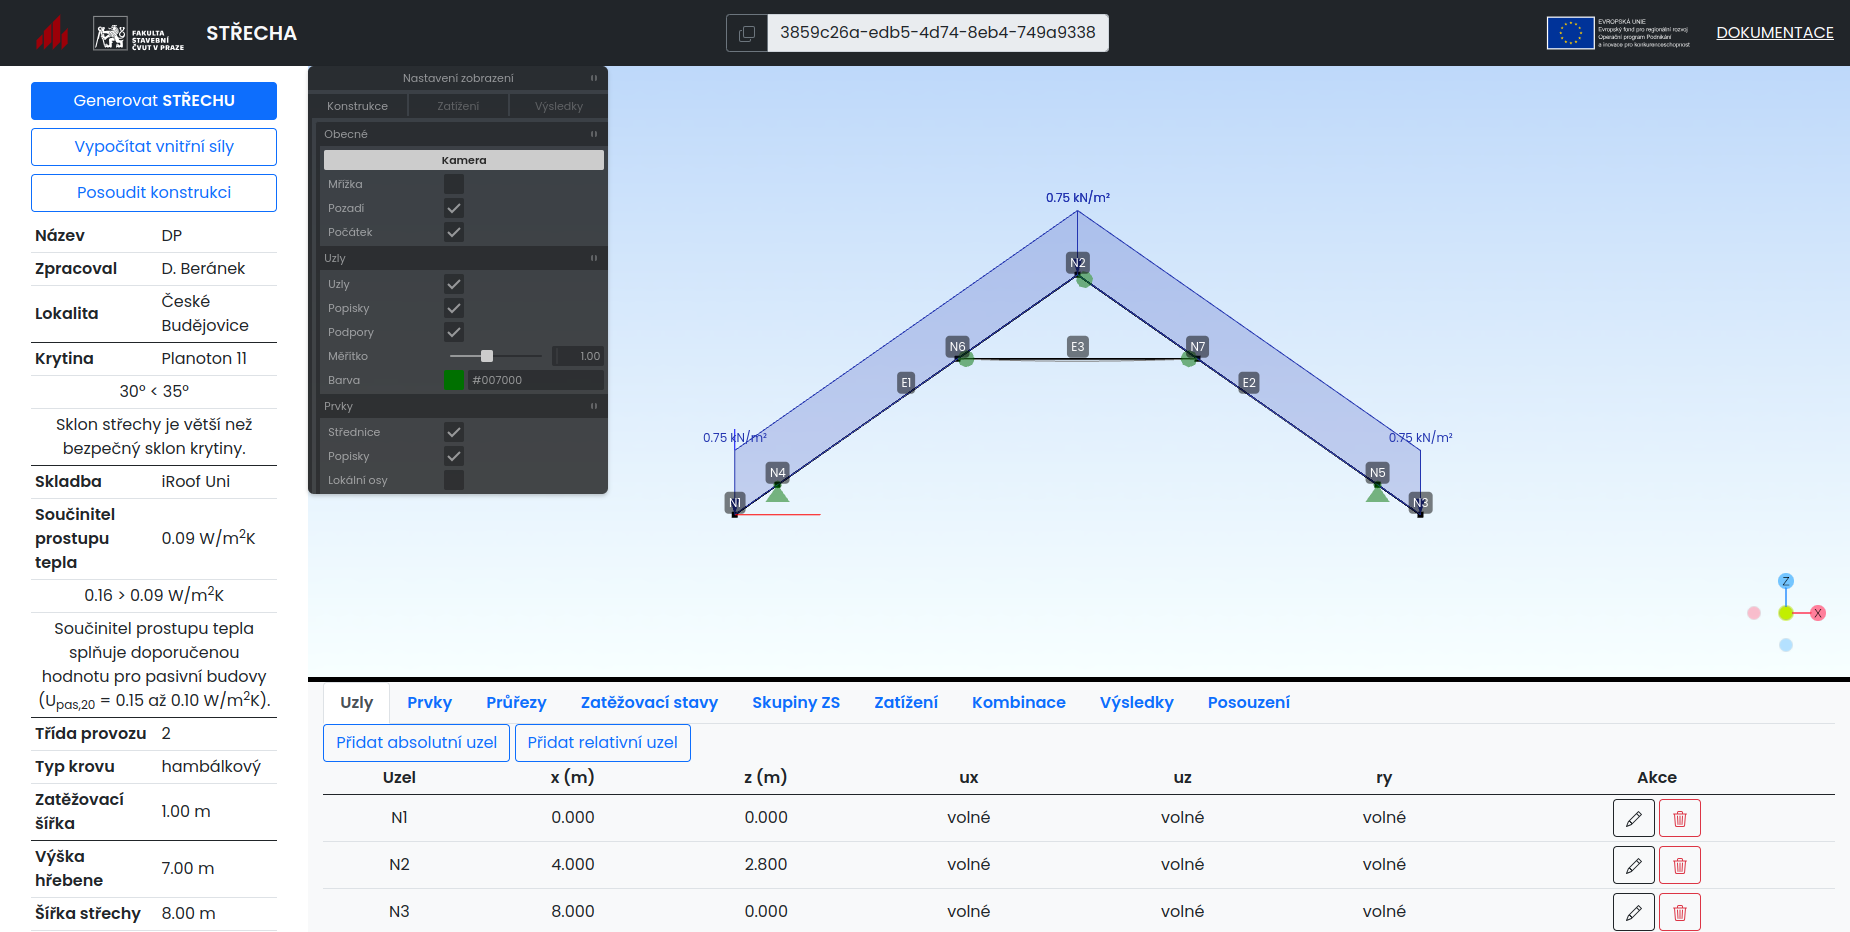
\includegraphics{assets/figures/wbapp/strecha_new.png}
    \caption{STŘECHA -- Nové uživatelské prostředí}
    \label{fig:roof_new}
\end{figure}

Na obrázku \autoref{fig:roof_new} je rozvržení nového uživatelského prostředí, na levé straně obrazovky se nachází panel s~informacemi o~projektu, jako je název, zpracovatel, lokalita, krytina, sklon střechy, skladba, součinitel prostupu tepla, typ krovu a další. V~hlavní části obrazovky se nachází vizualizace statického modelu, kde jsou zobrazeny uzly, prvky a aplikovaná zatížení. Uživatel může interaktivně přidávat, měnit a mazat uzly, prvky, zatížení a veškeré další objekty pomocí ovládacích prvků v~záložkách v~dolní části obrazovky. Tento přístup zajišťuje, že uživatelé mají přehled o~všech zadaných datech a mohou je snadno upravovat a kontrolovat.

\subsubsection*{Spodní panel}
V~dolní části obrazovky se nachází karty s~ovládacími prvky a přehlednými tabulkami, které zobrazují veškeré informace o~modelované konstrukci. Tyto karty zahrnují:
\begin{itemize}
    \item \textbf{Uzly}: Seznam všech uzlů v~modelu s~jejich souřadnicemi a definicí podepření v~jednotlivých směrech.
    \item \textbf{Prvky}: Seznam všech prvků, pro každý prvek se zde zobrazují jeho výchozí a koncový uzel, relativně zadané uzly, koncové klouby, délka a průřez.
    \item \textbf{Průřezy}: Seznam všech prvků s~definicí materiálu a základních geometrických veličin.
    \item \textbf{Zatěžovací stavy}: Seznam všech zatěžovacích stavů, jejich typ, kategorie, třída trvání zatížení a odpovídající součinitele podle ČSN EN 1990.
    \item \textbf{Skupiny ZS}: Skupiny zatěžovacích stavů, ze kterých se generují kombinace.
    \item \textbf{Zatížení}: Seznam spojitých a bodových zatížení na prvcích a v~uzlech. Na této kartě lze přepínat mezi zatěžovacími stavy. Zatížení pro aktivní zatěžovací stav se zobrazuje ve vizualizaci.
    \item \textbf{Kombinace}: Seznam všech kombinací, jejich mezní stav, typ a kombinační klíč.
    \item \textbf{Výsledky}: Seznam vnitřních sil ve všech průřezech, kde se může vyskytovat extrém vnitřních sil. Na této kartě lze přepínat mezi zatěžovacími stavy a kombinacemi zatížení. Pro aktivní výběr se vykreslují výsledky v~modelu.
    \item \textbf{Posouzení}: Přehled využití jednotlivých prutů.
\end{itemize}

Na každé kartě je tlačítko pro přidání nové entity do modelu. Zároveň lze každou entitu, kromě zatížení vlastní tíhou, vymazat nebo upravit.

\begin{figure}[H]
    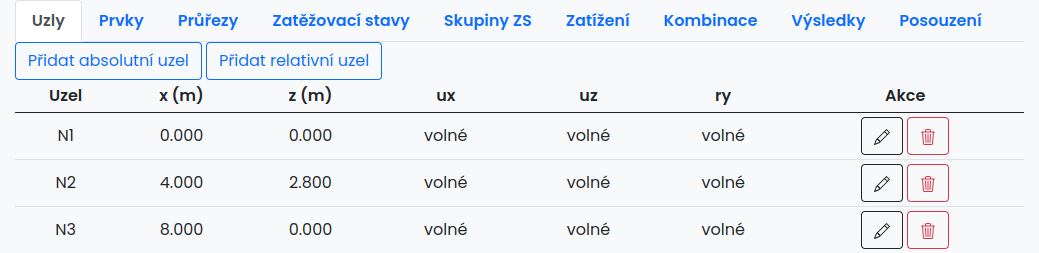
\includegraphics{assets/figures/wbapp/nodes_tab.png}
    \caption{STŘECHA -- Záložka s~uzly}
    \label{fig:nodes}
\end{figure}

\begin{figure}[H]
    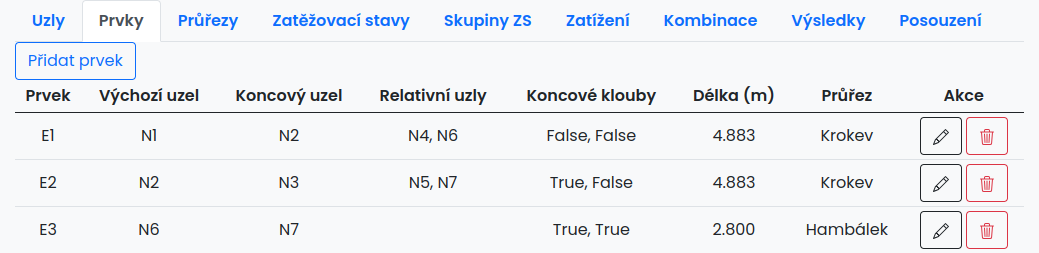
\includegraphics{assets/figures/wbapp/members_tab.png}
    \caption{STŘECHA -- Záložka s~prvky}
    \label{fig:members}
\end{figure}

\begin{figure}[H]
    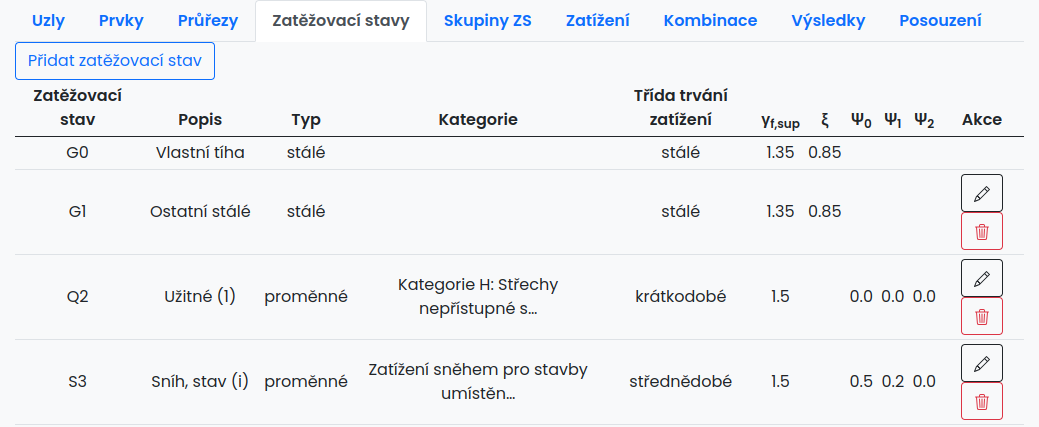
\includegraphics{assets/figures/wbapp/load_cases_tab.png}
    \caption{STŘECHA -- Záložka se zatěžovacími stavy}
    \label{fig:load_cases}
\end{figure}

\begin{figure}[H]
    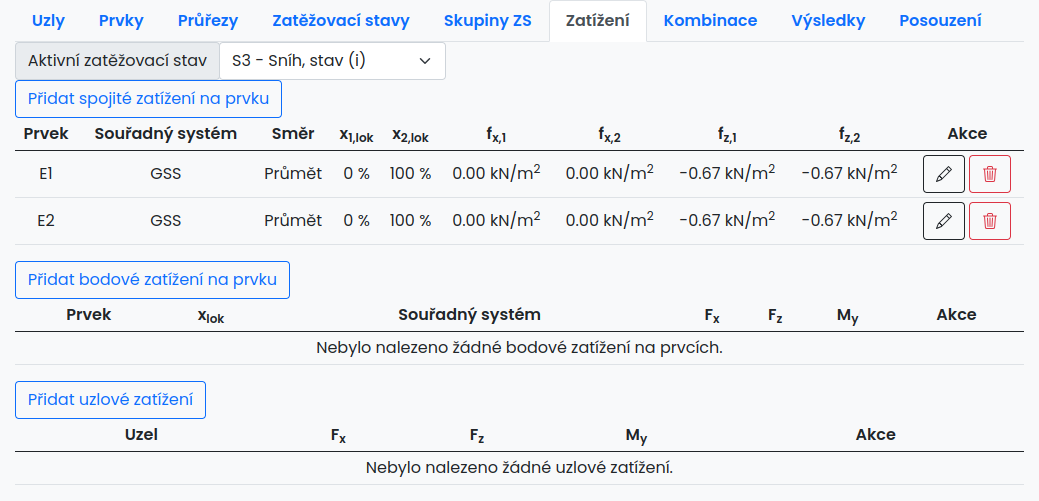
\includegraphics{assets/figures/wbapp/loads_tab.png}
    \caption{STŘECHA -- Záložka se zatížením}
    \label{fig:loads}
\end{figure}

\begin{figure}[H]
    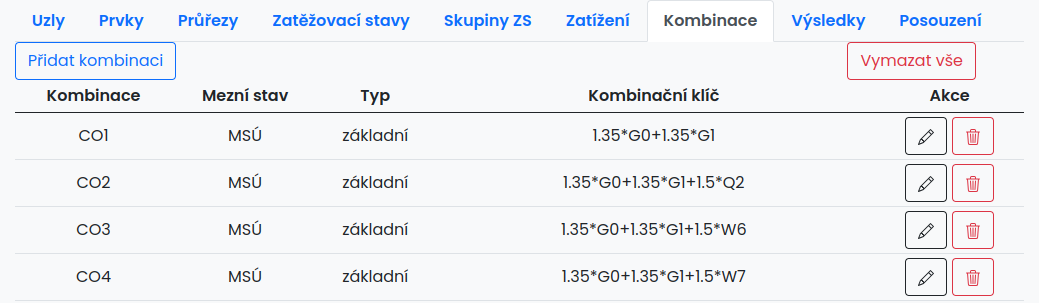
\includegraphics{assets/figures/wbapp/combos_tab.png}
    \caption{STŘECHA -- Záložka s~kombinacemi zatížení}
    \label{fig:combos_tab}
\end{figure}

\subsubsection*{Definování entit}
Téměř každou entitu lze editovat. Po kliknutí na tlačítko \textbf{Přidat} v~horní části karty nebo tlačítko \textbf{Editovat} na řádku s~entitou se zobrazí okno umožňující zadání potřebných údajů.
\begin{figure}[H]
    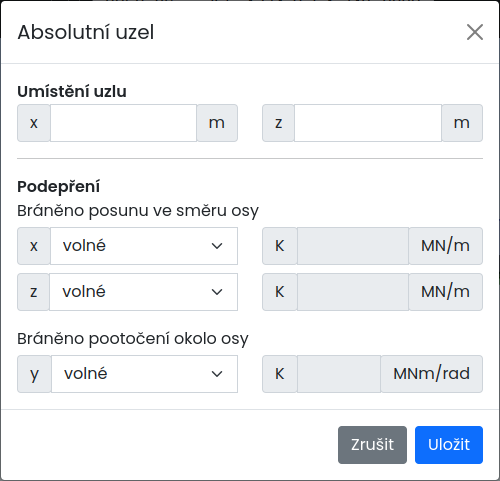
\includegraphics[width=7.5cm]{assets/figures/wbapp/add_node_modal.png}
    \caption{STŘECHA -- Okno pro přidání nového uzlu}
    \label{fig:add_node}
\end{figure}

\begin{figure}[H]
    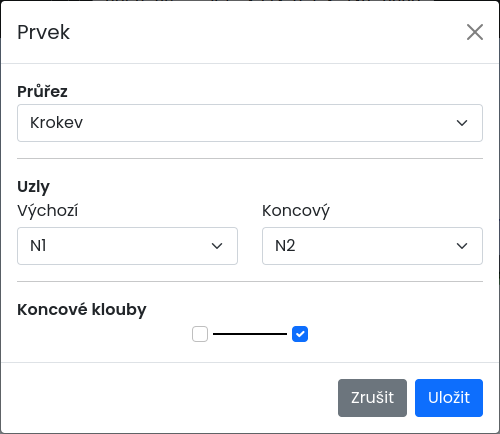
\includegraphics[width=7.5cm]{assets/figures/wbapp/add_member_modal.png}
    \caption{STŘECHA -- Okno pro přidání nového prvku}
    \label{fig:add_member}
\end{figure}

\begin{figure}[H]
    \includegraphics[width=7.5cm]{assets/figures/wbapp/add_load_Case_modal.png}
    \caption{STŘECHA -- Okno pro přidání nového zatěžovacího stavu}
    \label{fig:add_load_case}
\end{figure}

\subsection{Příklad}
Pro demonstraci schopností webové aplikace provedeme opět výpočet příkladu 5.2 ze \textit{Sbírky příkladů stavební mechaniky} \cite[Příklad 5.2]{sbirka_prikladu}, který byl již vypočítán v~kapitole \ref{sec:framesss_example}.

Protože v~aplikaci STŘECHA můžeme zadávat pouze dřevěné obdélníkové průřezy, musíme určit rozměry průřezu tak, abychom dosáhli stejné ohybové a normálové tuhosti průřezu. Použijeme dřevo třídy C24, pro které platí $\gls{E}_{m,0,k} = \SI{7,4}{\GPa}$. 

V~zadání příkladu je uvedeno, že Youngův modul pružnosti je $\gls{E} = \SI{30}{\GPa}$, moment setrvačnosti k~ose, kolem které jsou pruty namáhané ohybem $\gls{I_y} = \SI{1e-3}{\unit{\metre\tothe{4}}}$ a plochu $\gls{A}= \SI{4e-3}{{\metre\tothe{2}}}$.

Vyřešíme dvě rovnice pro dvě neznámé,
\begin{equation}
    \gls{E} \gls{I_y} = \gls{E}_{m,0,k} \frac{\gls{b}\gls{h}^{3}}{12},
\end{equation}
\begin{equation}
    \gls{E} \gls{A} = \gls{E}_{m,0,k} \gls{b} \gls{h}.
\end{equation}

Po vyřešení vychází $\gls{b} \approx \SI{9,362}{\mm}$ a $\gls{h} \approx \SI{1732}{\mm}$.

Z~následujících obrázků je patrné, že velikosti reakcí a průběhy vnitřních sil se přesně shodují s~průběhy uvedenými v~kapitole \ref{sec:framesss_example}.

Tento příklad lze otevřít zadáním unikátního idetifikačního kódu \texttt{0023d0bc-bc20-46b5-bfe7-dadc9bd10dfc}.

\begin{figure}[H]
    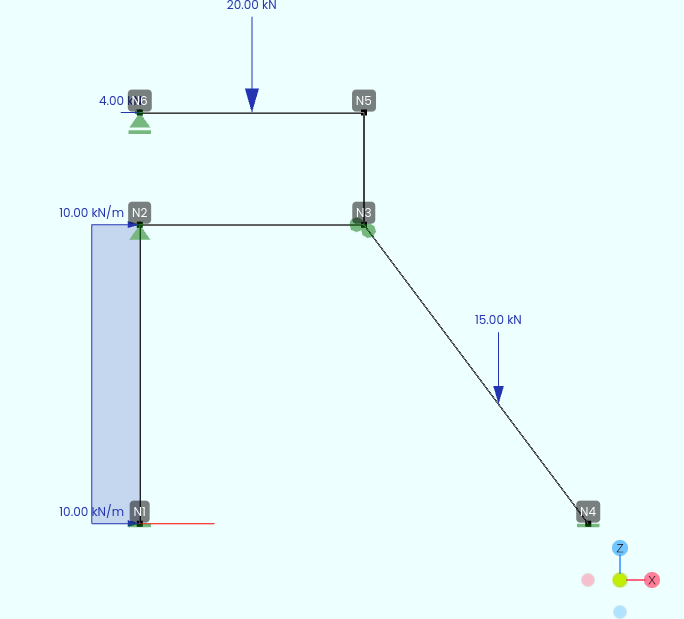
\includegraphics{assets/figures/wbapp/example/loads.png}
    \caption{Zatížení}
    \label{fig:wb_app_example_loads}
\end{figure}

\begin{figure}[H]
    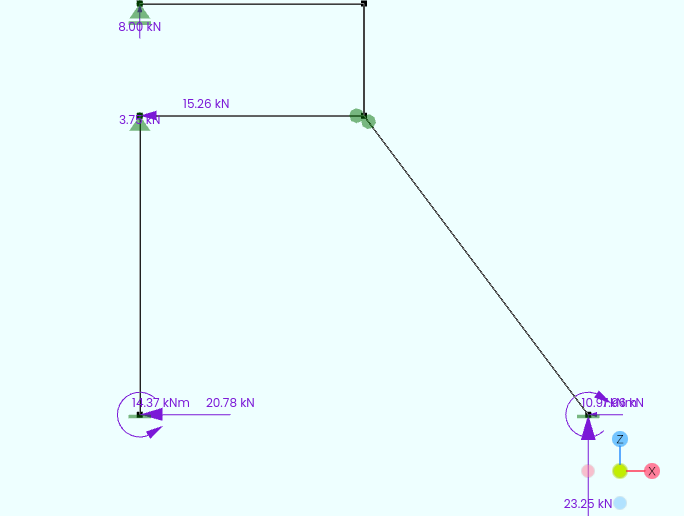
\includegraphics{assets/figures/wbapp/example/reactions.png}
    \caption{Reakce}
    \label{fig:wb_app_example_reactions}
\end{figure}

\begin{figure}[H]
    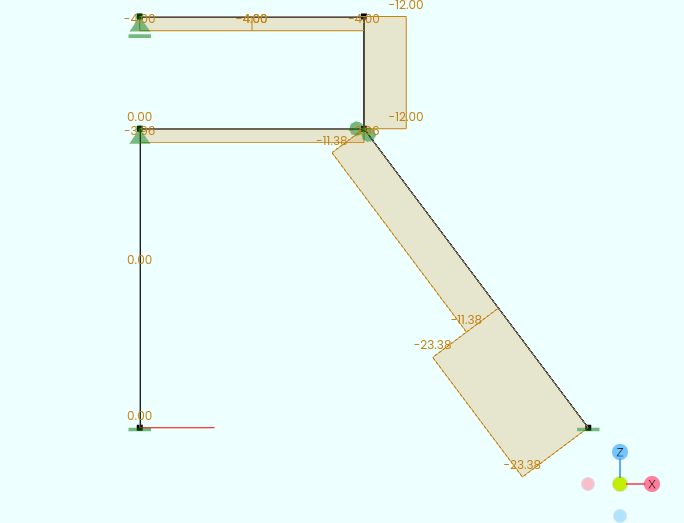
\includegraphics{assets/figures/wbapp/example/axial_force.png}
    \caption{Normálová síla}
    \label{fig:wb_app_example_axial}
\end{figure}

\begin{figure}[H]
    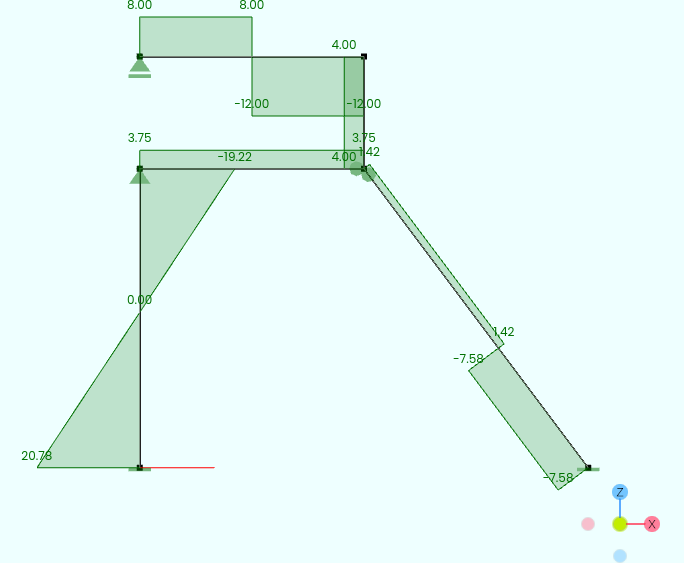
\includegraphics{assets/figures/wbapp/example/shear_force.png}
    \caption{Posouvající síla}
    \label{fig:wb_app_example_shear}
\end{figure}

\begin{figure}[H]
    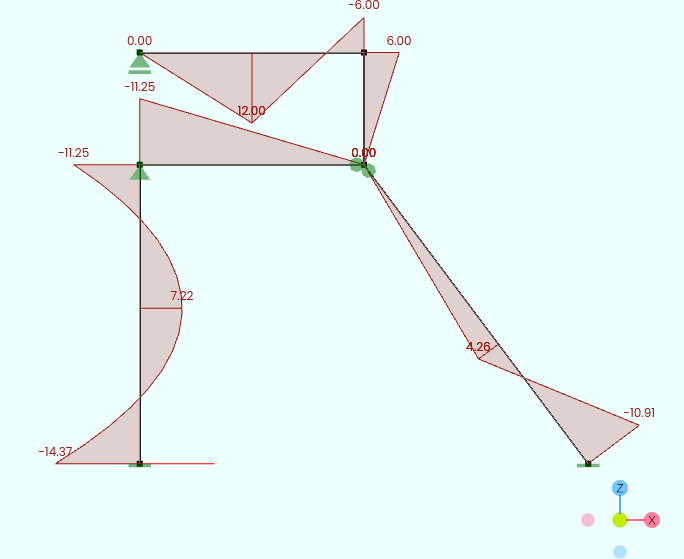
\includegraphics{assets/figures/wbapp/example/moments.png}
    \caption{Ohybové momenty}
    \label{fig:wb_app_example_moments}
\end{figure}

\section{Aplikace STROP}
Aplikace STROP je určená pro návrh a posouzení stropních konstrukcí Porotherm MIAKO, které jsou tvořené cihelnými vložkami MIAKO a keramobetonovými stropními trámy.

Pomocí aplikace lze posoudit stropní konstrukci, případně optimalizovat konstrukci na základě uživatelem definovaných parametrů.

V~rámci předchozí kapitoly bylo představeno integrování knihoven framesss a desssign do uživatelského rozhraní aplikace STŘECHA. V~rámci pokračující práce na představené webové aplikace budou tyto knihovny v~budoucnu integrovány i do aplikace STROP. Na následujících příkladech bude představen aktuální schopnosti aplikace a možnosti budoucího rozšíření a vylepšení.

\subsection{Prostý nosník}
Podle \cite[261]{PPN17} je maximální hodnota návrhového spojitého rovnoměrného zatížení (bez vlastní tíhy zmonolitněné konstrukce), kterou je možno na zmonolitněný strop přiložit, aby byla zachována požadovaná únosnost konstrukce pro beton třídy C20/25 a jednoduchý stropní trám POT 475 při tloušťce stropní konstrukce $\SI{250}{\milli\metre}$ a osové vzdálenosti trámů $\SI{625}{\milli\metre}$ rovna hodnotě $\SI{5,78}{\kilo\newton\per\metre\squared}$.
\begin{figure}[H]
    \begin{tikzpicture}
        \point{a}{0}{0};
        \point{b}{8}{0};
        \beam{1}{a}{b}[0][0];
        \support{1}{a};
        \support{2}{b};
        \lineload{1}{a}{b}[1];
        \dimensioning{1}{a}{b}{-1.5}[$\SI{4,65}{\metre}$];
        \notation{1}{a}{$\SI{5,78}{\kilo\newton\per\metre\squared}$}[above=1.5cm];
      \end{tikzpicture}
    \caption{Zadání příkladu}
    \label{fig:wb_app_strop_simple_beam}
\end{figure}

Na obr. \ref{fig:wb_app_schema} jsou zobrazeny hodnoty, které musíme vyplnit ve formuláři před odesláním dat k~výpočtu. Jedná se pouze o~statický obrázek.
\begin{figure}[H]
    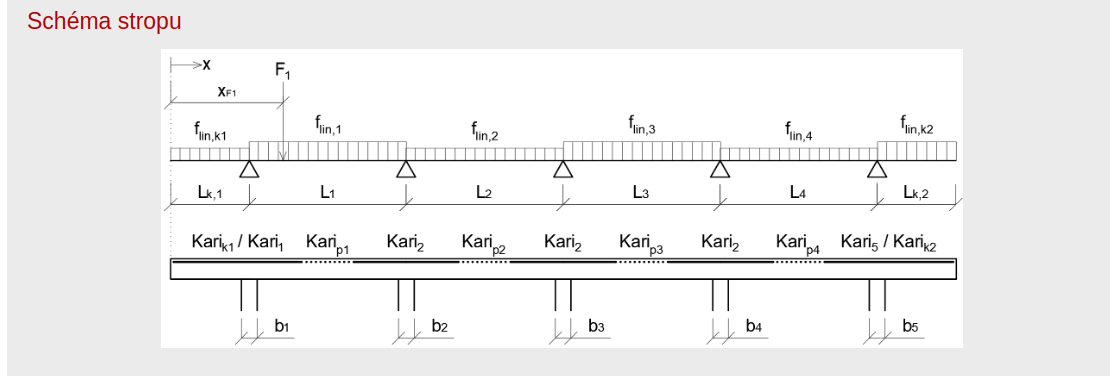
\includegraphics{assets/figures/wbapp/strop/00_schema.png}
    \caption{Schéma stropu}
    \label{fig:wb_app_schema}
\end{figure}

Nejprve je nutné definovat jednotlivá pole stropu. Z~obrázku \ref{fig:wb_app_pole_stropu} je patrné, že jediné nenulové pole je pole na druhém řádku.
\begin{figure}[H]
    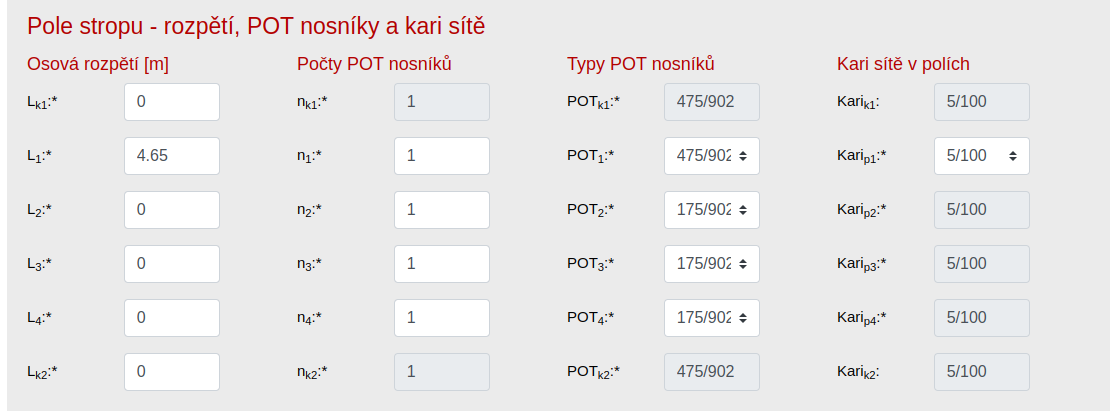
\includegraphics{assets/figures/wbapp/strop/01_pole.png}
    \caption{Pole stropu - rozpětí, POT nosníky a kari sítě}
    \label{fig:wb_app_pole_stropu}
\end{figure}

Tato část je určena především k~zadání nadpodporové výztuže. Protože nyní řešíme prostý nosník, nemusíme tuto část řešit.
\begin{figure}[H]
    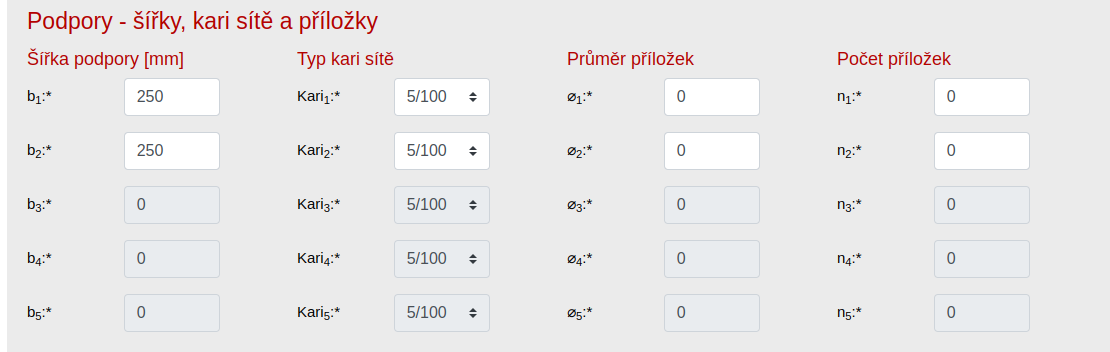
\includegraphics{assets/figures/wbapp/strop/02_podpory.png}
    \caption{Podpory - šířky, kari sítě a příložky}
    \label{fig:wb_app_podpory}
\end{figure}

V~další části definujeme průřez stropu, jak bylo zmíněno na začátku, jedná se o~strop tloušťky $\SI{250}{\milli\metre}$ s~osovou vzdáleností trámů $\SI{625}{\milli\metre}$.
\begin{figure}[H]
    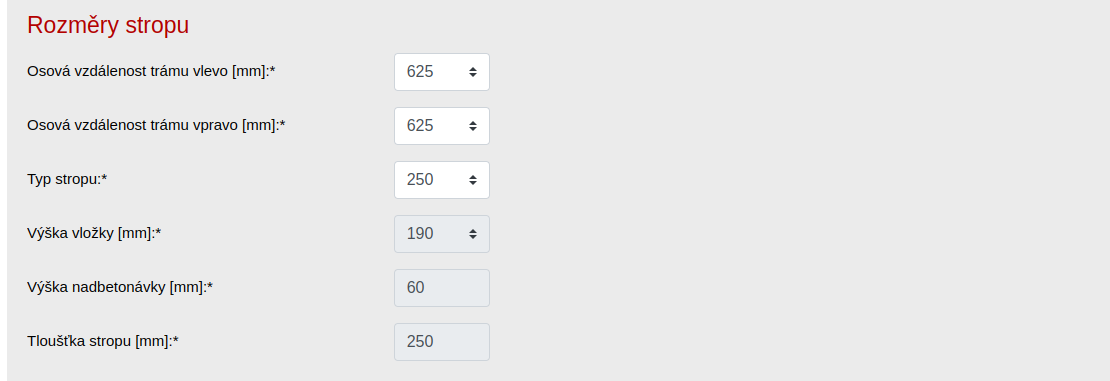
\includegraphics{assets/figures/wbapp/strop/03_rozmery.png}
    \caption{Rozměry stropu}
    \label{fig:wb_app_rozmery_stropu}
\end{figure}

Materiál uvažujeme jako beton C20/25. Protože řešíme mezní stav únosnosti, součinitel dotvarování betonu necháme na defaultní hodnotě.
\begin{figure}[H]
    
\includegraphics{assets/figures/wbapp/strop/04_material.png}
    \caption{Materiálové vlastnosti}
    \label{fig:wb_app_material}
\end{figure}

Dále zadáme přitížení stropu, lze zadat zatížení plošné (např. od podlahy, užitné zatížení) a liniové (např. příčka rovnoběžná s~osou nosníku). Pokud chceme, aby program vypočítal i průhyb, musíme vyplnit charakteristickou hodnotu. V~tomto případě si vystačíme s~hodnotou návrhovou. Přestože máme pouze jedno pole, na stránce se zobrazují šedě zabarvená okna pro ostatní pole.
\begin{figure}[H]
    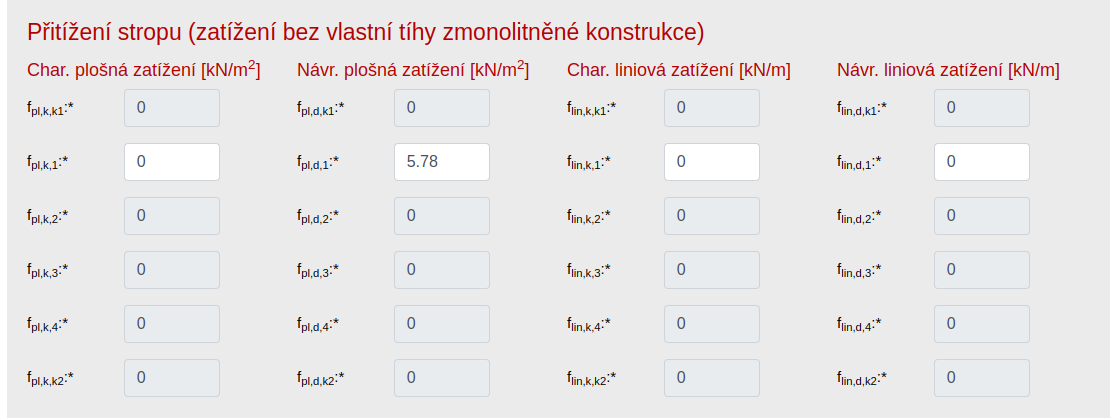
\includegraphics{assets/figures/wbapp/strop/05_pritizeni.png}
    \caption{Přitížení stropu (zatížení bez vlastní tíhy zmonolitněné konstrukce)}
    \label{fig:wb_app_pritizeni}
\end{figure}

V~další části lze zadat bodová zatížení, podobně jako u~plošného zatížení máme na výběr z~typu Sloup a typu Příčná stěna. Opět je nutné zadat zvlášť charakteristickou i návrhovou hodnotu. Tímto končí zadávání dat a je možné spustit výpočet pomocí tlačítka Spustit posouzení stropu.
\begin{figure}[H]
    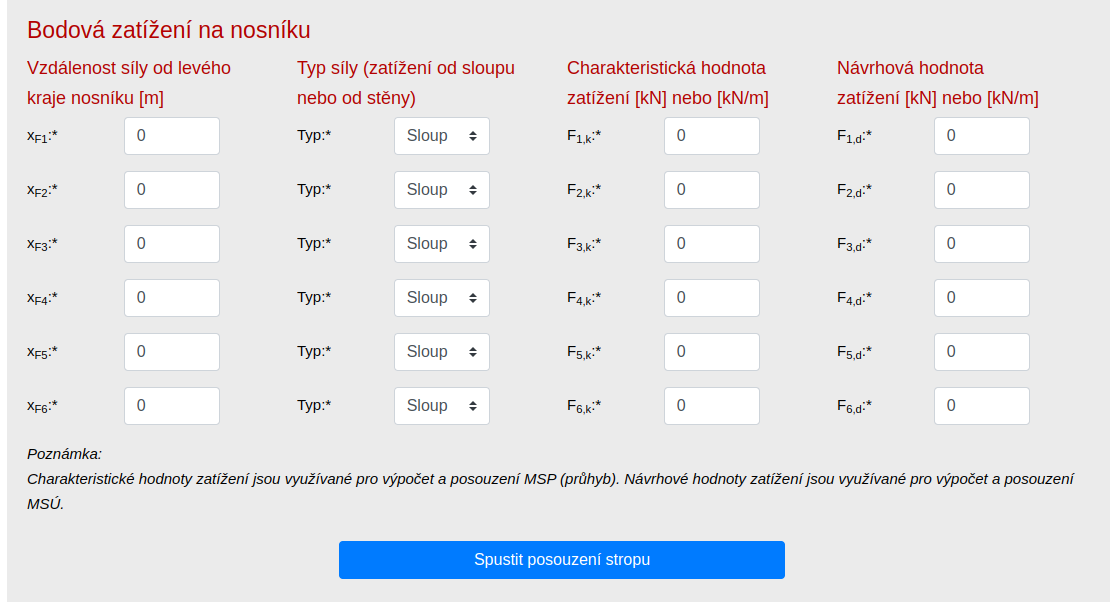
\includegraphics{assets/figures/wbapp/strop/06_bodova.png}
    \caption{Bodová zatížení na nosníku}
    \label{fig:wb_app_bodova}
\end{figure}

Po spuštění stropu server vygeneruje unikátní identifikační kód. Po kliknutí na tlačítko Přejít k~zobrazení výsledků posouzení budeme přesměrováni na stránku s~výsledky, která má identické pole jako stránka pro zadávání, rozdíl je však v~tom, že hodnoty už nelze upravovat, jsou zde pouze vypsané.
\begin{figure}[H]
    
\includegraphics{assets/figures/wbapp/strop/07_posouzeni.png}
    \caption{Výsledky posouzení}
    \label{fig:wb_app_posouzeni}
\end{figure}

Aplikace STROP zároveň vygeneruje statické obrázky, které jsou na stránce s~posouzením.
\begin{figure}[H]
    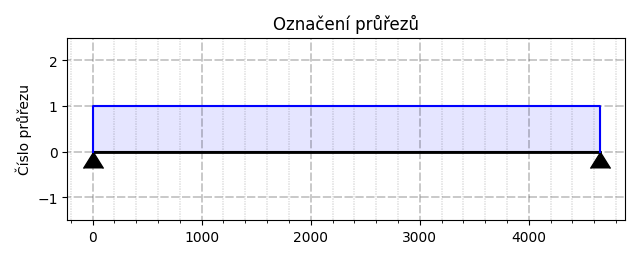
\includegraphics{assets/figures/wbapp/strop/08_prurezy.png}
    \caption{Označení průřezů po délce nosníku}
    \label{fig:wb_app_prurezy_cisla}
\end{figure}

\begin{figure}[H]
    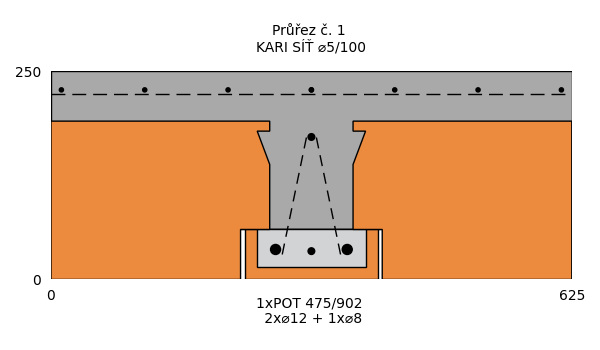
\includegraphics{assets/figures/wbapp/strop/09_prurez.png}
    \caption{Průřez stropní konstrukce}
    \label{fig:wb_app_prurez}
\end{figure}

\begin{figure}[H]
    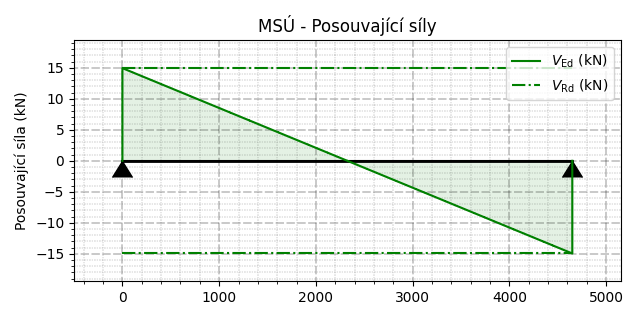
\includegraphics{assets/figures/wbapp/strop/10_shear.png}
    \caption{Posouvající síla}
    \label{fig:wb_app_shear}
\end{figure}

\begin{figure}[H]
    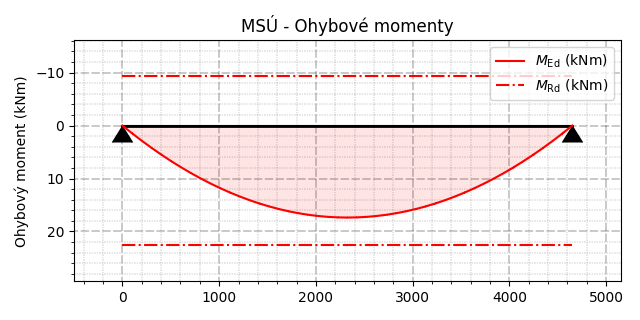
\includegraphics{assets/figures/wbapp/strop/11_moment.png}
    \caption{Ohybový moment}
    \label{fig:wb_app_moment}
\end{figure}

\begin{figure}[H]
    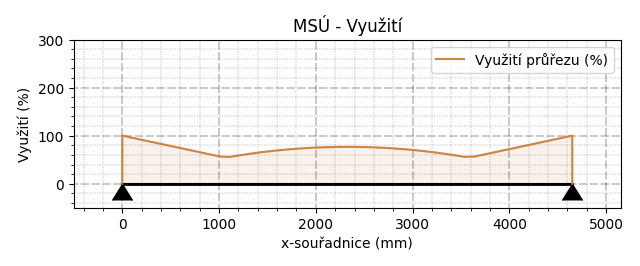
\includegraphics{assets/figures/wbapp/strop/12_vyuziti.png}
    \caption{Využití průřezů}
    \label{fig:wb_app_vyuziti}
\end{figure}

Z~obrázku \ref{fig:wb_app_vyuziti} je patrné, že konstrukce je využita na 100\%, což znamená, že program dává shodné výsledky s~tabulkou uvedenou v~\textit{Podkladu pro navrhování} \cite{PPN17}. 


